% !TeX encoding = UTF-8
% !TeX TS-program = xelatex
% !TeX spellcheck = en_GB
\documentclass[12pt,a4paper]{scrbook}

% Input Type and AMS-Packages
\usepackage{amsmath,amsfonts,amssymb,amsthm}
\usepackage{MnSymbol}
\usepackage{unicode-math}

% Typography
\usepackage{fontspec}
\setmainfont[Ligatures=TeX]{EB Garamond}
\newfontfamily\headingfont[RawFeature={+c2sc,+scmp},
                           Ligatures=TeX,
                           Letters=SmallCaps]{EB Garamond}
\setsansfont[Ligatures=TeX, Scale=MatchLowercase]{Open Sans}
\setmonofont[Scale=MatchLowercase]{Fira Mono}
\setmathfont[Scale=MatchUppercase]{STIX Two Math}
\setmathrm[Scale=MatchUppercase]{STIX Two Math}
\setmathtt[Scale=MatchUppercase]{Fira Mono}


\renewcommand{\scshape}{\headingfont}

\usepackage{polyglossia}
\setdefaultlanguage[variant=british]{english}
\setotherlanguage{german}
\usepackage{floatrow}
\usepackage{booktabs}

\usepackage[autostyle]{csquotes}
\usepackage{microtype}
\usepackage{enumitem}
\usepackage{subcaption}

\usepackage{letltxmacro}

\newlist{thmlist}{enumerate}{1}			% thmlist-s may only be used in theorem environments
\setlist[thmlist]{label=(\roman{thmlisti}),
                  ref=\thethm.(\roman{thmlisti}),
                  noitemsep}
\newlist{exlist}{enumerate}{1}
\setlist[exlist]{label=(\arabic{exlisti}),
                 ref=\thethm.(\arabic{exlisti}),
                 noitemsep,
                 leftmargin=0pt,
                 itemindent=2\parindent}
\newlist{plist}{enumerate}{1}
\setlist[plist]{label=(\roman{plisti}),
                ref=(\roman{plisti}),
                noitemsep,
                leftmargin=0pt,
                itemindent=2\parindent}
\newlist{clist}{enumerate}{2}
\setlist[clist]{label*=(\alph*),
                ref=(\alph*),
                noitemsep,
                leftmargin=0pt,
                itemindent=2\parindent}

\usepackage{setspace}
\renewcommand{\arraystretch}{1.5}

\usepackage[symbol]{footmisc}		% Use symbols for footnotes
\usepackage{perpage}				% Package to reset counters at the end of each page.
\MakePerPage{footnote}				% Reset footnote-counter at the end of each page

\usepackage{listingsutf8}	% Typeset code.
\lstset{extendedchars=true,
        basicstyle=\ttfamily,
        commentstyle=\color{gray},
        stringstyle=\color{darkgray},
        xleftmargin=\parindent,
        language=haskell}

% BibLaTex
\usepackage[style=numeric,backend=biber]{biblatex}
\addbibresource{./references.bib}


% Math, Operators and Theorems
\usepackage{thmtools}	% More Flexibility in Theorem Styles + Provides in Combination with ref-Packages the
						% Possibility to Refer to Theorem Style in Reference.
\usepackage{faktor}		% Displays factor groups

\numberwithin{equation}{section}

\DeclareMathOperator{\N}{\mathbb{N}}
\DeclareMathOperator{\Z}{\mathbb{Z}}
\DeclareMathOperator{\Q}{\mathbb{Q}}
\DeclareMathOperator{\R}{\mathbb{R}}
\DeclareMathOperator{\C}{\mathbb{C}}
\DeclareMathOperator{\F}{\mathbb{F}}

\DeclareMathOperator{\Aut}{Aut}
\DeclareMathOperator{\id}{id}

\DeclareMathOperator{\kernel}{ker}
\DeclareMathOperator{\im}{im}
\DeclareMathOperator{\End}{\mathrm{End}}
\DeclareMathOperator{\Hom}{\mathrm{Hom}}
\DeclareMathOperator{\Mod}{\mathrm{mod}}
\DeclareMathOperator{\D}{\mathrm{D}}
\DeclareMathOperator{\lcm}{\mathrm{lcm}}
\DeclareMathOperator{\ord}{\mathrm{ord}}

\newcommand{\sta}{\texttt{§}}
\newcommand{\emp}{\texttt{\_}}
\newcommand{\zer}{\mathtt 0}
\newcommand{\one}{\mathtt 1}
\newcommand{\state}[1]{s_{\text{#1}}}
\newcommand{\sstart}{\state{start}}
\newcommand{\shalt}{\state{halt}}
\newcommand{\scheck}{s_{\text{check}}}
\newcommand{\enc}[1]{\ulcorner #1 \urcorner}
\newcommand{\rel}[1]{\mathrel{\MakeUppercase #1}}
\newcommand{\algint}[1][K]{\mathcal{O}_{#1}}


\declaretheoremstyle[
    spaceabove=6pt, spacebelow=6pt,
    headfont=\headingfont,
    notefont=\mdseries, notebraces={(}{)},
    bodyfont=\itshape,
    postheadspace=0.5\parindent
    ]{mythm}
\declaretheoremstyle[
    spaceabove=6pt, spacebelow=6pt,
    headfont=\headingfont,
    notefont=\mdseries, notebraces={(}{)},
    bodyfont=\normalfont,
    postheadspace=0.5\parindent
    ]{mydef}

\declaretheorem[
	name=Theorem,
    style=mythm,
  	refname={theorem,theorems},		%Lower Case Versions of Theorem Type
  	Refname={Theorem,Theorems},
  	numberwithin=section]{thm}
\declaretheorem[
	name=Lemma,
    style=mythm,
	refname={lemma,lemmas},
	Refname={Lemma,Lemmas},
	sibling=thm]{lem}
\declaretheorem[
	name=Proposition,
    style=mythm,
	refname={proposition,propositions},
	Refname={Proposition,Propositions},
	sibling=thm]{pro}
\declaretheorem[
	name=Corollary,
    style=mythm,
	refname={corollary,corollarys},
	Refname={Corollary,Corollarys},
	sibling=thm]{cor}

\declaretheorem[
	name=Definition,
	style=mydef,
	numbered=no]{defin}
\declaretheorem[
	name=Example,
	style=mydef,
	sibling=thm]{exam}

\declaretheorem[
	name=Remark,
	style=remark,
	numbered=no]{rem}



%\newtheorem{theo}{Theorem}[section]
%\newtheorem{lemma}[theo]{Lemma}
%\newtheorem{prop}[theo]{Proposition}
%\newtheorem{cor}[theo]{Corollary}
%\theoremstyle{definition}
%\newtheorem*{defin}{Definition}
%\newtheorem*{exam}{Example}
%\theoremstyle{remark}
%\newtheorem*{rem}{Remark}

%TikZ and TikZ-Styles
\usepackage{tikz}


% New- and Renewcommands

\newcommand{\seq}[2][n]{#2_{1},\ldots,#2_{#1}}
\newcommand{\nicefrac}[2]{#1/#2}
\newcommand{\set}[1]{\left\lbrace #1 \right\rbrace}




% ----------------------------------------------------------
% Only for drafts!
\usepackage{todonotes}
\usepackage{showlabels}	%Used in Drafts to Print references.
%-----------------------------------------------------------



% References
\usepackage{hyperref}
\usepackage[capitalize]{cleveref}

\hypersetup{
	pdftitle={On Hilbert's Tenth Problem over Rings of Algebraic Integers},
	pdfauthor={Tim Benedikt Herbstrith}}

%\Crefname{thm}{Theorem}{Theorems}
%\Crefname{lem}{Lemma}{Lemmas}
%\Crefname{pro}{Proposition}{Propositions}
%\Crefname{cor}{Corollary}{Corollaries}

%\crefname{thm}{thm.}{thms.}
%\crefname{lem}{lemma}{lemmas.}
%\crefname{pro}{prop.}{props.}
%\crefname{cor}{cor.}{cors.}

\Crefname{thm}{Thm}{Thms}
\Crefname{lem}{Lem.}{Lem.}
\Crefname{pro}{Prop.}{Props}
\Crefname{cor}{Cor.}{Cors}
\Crefname{exam}{Example}{Examples}

\addtotheorempostheadhook[thm]{\crefalias{thmlisti}{thm}}
\addtotheorempostheadhook[lem]{\crefalias{thmlisti}{lem}}
\addtotheorempostheadhook[pro]{\crefalias{thmlisti}{pro}}
\addtotheorempostheadhook[cor]{\crefalias{thmlisti}{cor}}
\addtotheorempostheadhook[exam]{\crefalias{exlisti}{exam}}

%------------------------------------------------------------------------------------------------------------------

\begin{document}

% Using Layers in TikZ
\pgfdeclarelayer{background}
\pgfsetlayers{background,main}

% Page Breaks for Displayed Formulas
\allowdisplaybreaks

\frontmatter

% !TeX encoding = UTF-8
% !TeX TS-program = xelatex
% !TeX spellcheck = en_GB
% !TeX root = ../Herbstrith-H10_over_AI.tex

\begin{titlepage}
%\vspace*{-2cm}  % bei Verwendung von vmargin.sty
\begin{flushright}
    \includegraphics{uni-logo}
\end{flushright}
\vspace{0.5cm}

\begin{center}  % Diplomarbeit ODER Magisterarbeit ODER Dissertation
    \Huge{\textsf{\textbf{\MakeUppercase{
        Masterarbeit
    }}}}
    \vspace{1.5cm}

    \large{\textsf{  % Diplomarbeit ODER Magisterarbeit ODER Dissertation
                     % (Dies ist erst die Ueberschrift!)
        Titel der Masterarbeit
    }}
    \vspace{.1cm}

    \LARGE{\textsf{ On Hilbert's Tenth Problem over\\
                    Rings of Algebraic Integers
    }}
    \vfill

    \large{\textsf{  % Verfasserin ODER Verfasser (Ueberschrift)
        Verfasser
    }}

    \Large{\textsf{  Tim Benedikt Herbstrith
    }}
    \vfill

    \large{\textsf{
        angestrebter akademischer Grad  % (Ueberschrift)
    }}

    \Large{\textsf{  % Magistra ODER Magister ODER Doktorin ODER Doktor
                     % ACHTUNG: Kuerzel "Mag.a" oder "Dr.in" nicht zulaessig
        Master of Science (MSc.)
    }}

\vspace{1.5cm}

\noindent\textsf{Wien, im Monat Mai 2018}  % <<<<< ORT, MONAT UND JAHR EINTRAGEN
\vfill

\noindent\begin{tabular}{@{}ll}
\textsf{Studienkennzahl lt.\ Studienblatt:}
&
\textsf{A 033 821}  % <<<<< STUDIENKENNZAHL EINTRAGEN
\\
    % BEI DISSERTATIONEN:
%\textsf{Dissertationsgebiet lt. Studienblatt:}
    % ANSONSTEN:
\textsf{Studienrichtung lt.\ Studienblatt:}
&
\textsf{Mathematik}  % <<<<< DISSGEBIET/STUDIENRICHTUNG EINTRAGEN
\\
% Betreuerin ODER Betreuer:
\textsf{Betreuer: }
&
\textsf{ao.~Univ.-Prof.~Mag.~Dr.~Ch.~Baxa}  % <<<<< NAME EINTRAGEN
\end{tabular}
\end{center}
\end{titlepage}

\newpage%
\thispagestyle{empty}%
\vspace*{\fill}%
\noindent%
\begin{footnotesize}%
If not stated otherwise, the text of \emph{On Hilbert's Tenth Problem over Rings
of Algebraic Integers} by Tim B. Herbstrith is licenced under a \textsc{Creative
Commons Attribution-NonCommercial-ShareAlike 4.0 International License}. All
code snippets are provided `as is' without warranty of any kind, express or
implied, including but not limited to the warranties of merchantability, fitness
for a particular purpose and non-infringement under the terms of the
\textsc{MIT} licence. The source codes and the aforementioned licences are
published at
\begin{center}
 \url{https://github.com/tim6her/h10-over-rings-of-integers}
\end{center}
\end{footnotesize}
\cleardoublepage


\begin{german}
\section*{Vorwort}
\todo{Schreibe das Vorwort}
\end{german}

\vspace{1.5cm}

\section*{Abstract}
\todo{Write the abstract}
\newpage
\thispagestyle{empty}
\tableofcontents


\mainmatter
%\onehalfspacing

\chapter{Prerequisites and central notions}

Before stating Hilbert's 10th problem and proving its undecidability in
certain rings of algebraic integers, we remind the reader on some
notions from theoretical computer science and number theory, as well as
fix some notations.

\section{Prerequisites from theoretical computer science}
% !TeX encoding = UTF-8
% !TeX TS-program = xelatex
% !TeX engine=xelatex
% !TeX spellcheck = en_GB
% !TeX root = ../Herbstrith-H10_over_AI.tex

In this section I closely follow the lecture notes on the subject by
\textcite{Mueller2016}.

\begin{defin}
  A \emph{(decision) problem} is a subset of the set of finite
  $\zer$-$\one$-strings $\lbrace \zer, \one \rbrace^*$ including the
  empty string $λ$. One calls $\lbrace \zer, \one \rbrace$
  \emph{alphabet} and its elements \emph{bits.}
\end{defin}

One immediate objection against this definition is that not all problems
arise as subsets of these strings. However, such problems $Q$ are
captured up to an encoding.

\[ \enc{\cdot} : Q → \lbrace \zer, \one \rbrace^*\]

One usually does not concern oneself with the details of this encoding.
However, the encoding should capture the structure of the problem---a notion
that will be made precise in \cref{sec:computable structures}.

\begin{exam}
  Consider the problem of deciding whether a finite simple graph is
  connected or not. If one demands the vertex set to be of the form
  $\set{0, 1, …, n}$, then the set of all graphs can be encoded
  as the set of the respective adjacency matrices written as a string

  \[b_{00}b_{01} …b_{0n}b_{10}…b_{nn}\]

  of length $(n + 1)^2$, where $b_{ij} = \one$ if and only if the
  vertices $i$ and $j$ are connected.
\end{exam}

\begin{defin}
  A \emph{Turing machine} $\mathbb A$ on the \emph{alphabet}
  $A = \lbrace \sta, \emp, \zer, \one \rbrace$ is a tuple $(S, δ)$,
  where $\sstart, \shalt ∈ S$ is a finite non-empty set, called
  \emph{set of states}, and

  \[δ: S × A → S × A × \lbrace -1, 0, 1 \rbrace\]

  is called \emph{transition function}. If $δ(s, a) = (s', b, m)$, one
  demands that the following axioms are satisfied

  \begin{thmlist}
  \item
    $a = \sta$ if and only if $b = \sta$,
  \item
    If $a = \sta$, then $m ≠ -1$, and
  \item
    If $s = \shalt$, then $s' = \shalt$, $a = b$ and $m = 0$.
  \end{thmlist}
\end{defin}

Informally, one can think of a Turing machine as a device, consisting of a
\emph{work-tape} and a \emph{head}. The work-tape stores all the information in
cells arranged in a consecutive order. Each of these cells contains a letter
from the alphabet.

Let us look at the example of the Turing machine in \cref{fig:Turing machine}.
During the run of the machine the head reads the symbol $\zer$ at the current
position and the machine evaluates the transition function $δ$ at $\zer$ and the
current state $\state{overflow}$. Now assume that

\[ δ(\state{overflow}, \zer) = (\state{return}, \one, -1). \]

One interprets this in the following way. The Turing machine changes its state
to $\state{return}$, the head writes $\one$ in the current cell and moves one
cell to the left. The movement is determined by the last item of the triple
$δ(\state{overflow}, \zer)$, where $-1$ indicates moving to the left, $1$
indicates moving to the right, and $0$ indicates not moving at all.

\begin{figure}
  \includegraphics{res/turing_add1_4}
  \caption{A Turing machine}
  \label{fig:Turing machine}
\end{figure}

\begin{defin}
  Let $\mathbb A = (S, δ)$ be a Turing machine. A \emph{configuration}
  of $\mathbb A$ is a triple $(s, j, c) ∈ S × ℕ × A^ℕ$. It reflects
  the current state of $\mathbb A$, the current position of its
  head, and the content of its work-tape.
\end{defin}

A configuration of the form $(\shalt, 0, c)$ is called \emph{halting}. A
\emph{start configuration} is of the form $(\sstart, 0, c)$ such that $c(0) =
\sta$ and there exists an $n ∈ ℕ$ such that $c(i) = \emp$ if and only if $i >
n$. This means that in a start configuration the work-tape reads

\[\sta x_1 x_2 … x_n \emp \emp …\]

It will be very convenient to identify the finite string $x_1…x_n$ with this
tape content.

\begin{defin}
  One writes $(s, j, c) \vdash_1 (s', j', c')$ and calls $(s', j', c')$ a
  \emph{successor configuration} of $(s, j, c)$ if there exists an $m ∈ \lbrace
  -1, 0, 1 \rbrace$ such that

  \begin{itemize}
  \item
    $δ(s, c) = (s', c', m)$,
  \item
    $j' = j + m$, and
  \item
    $c'(ℓ) = c(ℓ)$ for all $ℓ ≠ j$.
  \end{itemize}

  This relation makes the set of all configurations of $\mathbb A$ into a
  directed graph. A \emph{run} of $\mathbb A$ on $x$ is a path in this directed
  graph starting at the start configuration $(\sstart, 0, x)$. A run of
  $\mathbb A$ on $x$ is \emph{halting} or \emph{complete} if it reaches a
  halting configuration $(\shalt, 0, y)$. In this case I write $\mathbb A (x) =
  y$.
\end{defin}

I will denote Turing machines using listings, where the fact that
$δ_\text{delta} (\state{state}, b) = (\state{state'}, c, m)$ is encoded by

\begin{lstlisting}
delta "state" c = ("state'", c', m)
\end{lstlisting}

Variables \verb+c+ match all possible states or characters in the alphabet
respectively. However, I follow the convention that if an assignment of
variables matches more than one pattern, the first matching pattern is chosen.
This means that
%
\begin{lstlisting}
delta "state" 1 = ("state'", 1, 1)
delta "state" c = ("state''", c, 0)
\end{lstlisting}
%
should be interpreted as
%
\[ δ(s, c) =
  \begin{cases}
    (\state{state'}, \one, 1) & \text{if } s=\state{state} ∧ c = \one\\
    (\state{state''}, c, 0) & \text{if } s=\state{state} ∧ c ≠ \one
  \end{cases}.
\]

See \cref{app:turing} on how to simulate Turing machines
using the \emph{Haskell} programming language.

\begin{exam}
    Consider the Turing machine $\mathbb A_\text{add1} = (\lbrace \sstart,
    \shalt, \state{overflow}, \state{return}, \state{error} \rbrace,
    δ_\text{add1})$ that adds $1$ to a (possibly zero-patched) binary
    representation of a natural number $n$. Its transition function is described
    in \cref{lst:add1}. The last line of the program ensures, that $δ$ is a
    complete function, as it matches all remaining pairs of states and
    characters and lets the machine enter the state $\state{error}$. The
    complete run of $\mathbb A_\text{add1}$ on $\one\one\zer\one$ can be seen in
    \cref{fig:complete run}.
\end{exam}

\lstinputlisting[float, frame=tb,
                 caption=A Turing machine adding one to the input string,
                 label=lst:add1]{./listings/add1.hs}

\begin{figure*}
    \begin{subfigure}{.5\textwidth}
        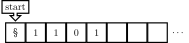
\includegraphics{res/turing_add1_1}
        \caption{$δ(\sstart, \sta) = (s_\text{overflow}, \sta, 1)$}
    \end{subfigure}

    \begin{subfigure}{.5\textwidth}
        \includegraphics{res/turing_add1_2}
        \caption{$δ(s_\text{overflow}, \one) = (s_\text{overflow}, \one, 1)$}
    \end{subfigure}

    \begin{subfigure}{.5\textwidth}
        \includegraphics{res/turing_add1_3}
        \caption{$δ(s_\text{overflow}, \one) = (s_\text{overflow}, \one, 1)$}
    \end{subfigure}

    \begin{subfigure}{.5\textwidth}
        \includegraphics{res/turing_add1_4}
        \caption{$δ(s_\text{overflow}, \zer) = (s_\text{return}, \one, -1)$}
    \end{subfigure}

    \begin{subfigure}{.5\textwidth}
        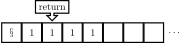
\includegraphics{res/turing_add1_5}
        \caption{$δ(s_\text{return}, \one) = (s_\text{return}, \one, -1)$}
    \end{subfigure}

    \begin{subfigure}{.5\textwidth}
        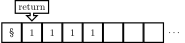
\includegraphics{res/turing_add1_6}
        \caption{$δ(s_\text{return}, \one) = (s_\text{return}, \one, -1)$}
    \end{subfigure}

    \begin{subfigure}{.5\textwidth}
        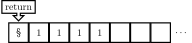
\includegraphics{res/turing_add1_7}
        \caption{$δ(s_\text{return}, \sta) = (s_\text{halt}, \sta, 0)$}
    \end{subfigure}

    \begin{subfigure}{.5\textwidth}
        \includegraphics{res/turing_add1_8}
        \caption{$δ(s_\text{halt}, \sta) = (s_\text{halt}, \sta, 0)$}
    \end{subfigure}

    \caption{The complete run of $\mathbb A_\text{add1}$ on $\one\one\zer\one$}
    \label{fig:complete run}
\end{figure*}

\begin{defin}
    Let $\mathbb A$ be a Turing machine.

    \begin{thmlist}
        \item
          $\mathbb A$ \emph{computes} the partial function that maps each
          $x$ with a complete run to $\mathbb A(x)$ and is undefined for all
          other strings.
        \item
          $\mathbb A$ \emph{accepts} all $x$ such that
          $\mathbb A(x) = \one$ and \emph{rejects} them if
          $\mathbb A(x) = \zer$.
        \item
          A partial function on $\lbrace \zer, \one \rbrace^*$ is
          \emph{computable} if there is a Turing machine computing it. Sometimes
          computable functions are referred to as \emph{recursive} or
          \emph{efficient} functions.
        \item
          A subset of $\lbrace \zer, \one \rbrace^*$, i.e. a
          problem, is \emph{decidable} if there is a Turing machine computing
          its characteristic function.
        \item
          A problem is called \emph{semi-decidable} or \emph{computably
          enumerable} if there is a Turing machine accepting precisely the
          elements of the problem.
    \end{thmlist}
\end{defin}

The last item of the definition above means that a problem is
semi-decidable if there is a Turing machine affirming membership of the
corresponding set but it might not be able to refute membership.

Note that every finite problem is decidable by a Turing machine that reads the
tape content and checks at every step whether there are elements in the problem
that start with the tape content the machine has read. After $n + 1$ steps,
where $n$ denotes the length of the longest string in the problem, the machine
stops at the latest.

\begin{lem} \label{lem:composition of Turing machines}
  Let $\mathbb A_1 = (S_1, δ_1)$ and $\mathbb A_2 = (S_2, δ_2)$ be Turing
  machines computing $f_1: D_1 → \set{\zer, \one}^*$ and $f_2: D_2 → \set{\zer,
  \one}^*$ respectively ($D_1, D_2 \subseteq \set{\zer, \one}^*$). Then there
  exists a Turing machine $\mathbb A_{f_2 \circ f_1}$ computing the partial
  function $f_2 \circ f_1: D_1 ∩ f_1^{-1}(D_2) → \set{\zer, \one}^*$ obtained by
  composing $f_1$ and $f_2$.
\end{lem}
\begin{proof}
  One constructs $\mathbb A_{f_2 \circ f_1}$ from $\mathbb A_1$ and $\mathbb
  A_2$ as follows. Let $S_1 = \set{\sstart, \shalt} \sqcup S_1'$ and $S_2 =
  \set{\sstart, \shalt} \sqcup S_2'$, then set $S = \set{\sstart, \shalt} \sqcup
  S_1' \sqcup S_2' \sqcup \set{\state{compose}}$, where $\sqcup$ denotes the
  disjoint union. Now set for $c ∈ A$
  %
  \begin{align*}
    δ (s, c) &=
      \begin{cases}
        δ_1 (s, c) & \text{if } s ∈ S_1' ∪ \set\sstart \\
        (\state{compose}, c', m) & \text{if } s ∈ S_1 \text{ and } δ_1(s, c) = (\shalt, c', m)\\
        δ_2 (s, c) & \text{if } s ∈ S_2' ∪ \set\shalt \\
      \end{cases}, \\
    δ (\state{compose}, c) &= δ_2 (\sstart, c).
  \end{align*}
  %
  Then $\mathbb A_{f_2 \circ f_1} = (S, δ)$ computes $f_1 \circ f_2$ because $δ$
  is defined to first run the program of $\mathbb A_1$ and if this machine would
  reach a halting state run $\mathbb A_2$.
\end{proof}
% IDEA
\todo{Maybe: A semi-decidable set is decidable iff its complement is semi-decidable}

\begin{exam}
    One can encode a natural number $n$

    \begin{exlist}
    \item \label{ex:tally encoding}
      in tally notation
      \begin{align*}
        n & ↦ \underbrace{\one…\one}_{n\text{-times}}, \quad \text{if } n > 0 \\
        0 & ↦ λ
      \end{align*}
    \item
      by its binary representation
      \begin{align*}
          n = 2^k + \sum_{i = 0}^{k-1} b_i 2^i & ↦ b_0…b_{k-1}\one, \quad
              \text{if } n > 0\\
                                             0 & ↦ \zer,
      \end{align*}
      or
    \item \label{ex:omega encoding}
      by a shifted and truncated form of its binary representation
      \begin{align*}
        n = 1 + \sum_{i = 0}^k b_i 2^i & ↦ b_0…b_k, \quad \text{if } n > 0\\
                                     0 & ↦ λ
      \end{align*}

      In other words, $n$ is mapped to the $n$-th string if one orders $\lbrace
      \zer, \one \rbrace ^ ℕ$ lexicographically. Following an tradition in
      logics I denote $ℕ$ under this last encoding by $ω$.
    \end{exlist}

    In either case the set obtained by encoding $ℕ$ is easily seen to be
    decidable. In the first case, check that the string contains only copies
    of the bit $\one$. Indeed, this can be achieved by the Turing machine
    %
    \[\mathbb A_\text{tally} =
      ( \lbrace \sstart, \shalt, \scheck, \state{accept}, \state{reject},
        \state{rejectMR}, \state{error} \rbrace, δ),\]
    %
    whose transition function is displayed in \cref{lst:tally encoding}.

    In the second case it suffices to check that the string has length $1$
    or ends in an $\one$, and in the third case every string is accepted.
\end{exam}

\lstinputlisting[float, frame=tb,
                 caption=A Turing machine checking whether the input is tally-encoded,
                 label=lst:tally encoding]{./listings/tally.hs}

Taking another look at the definition of computability, one sees that only unary
functions defined on subsets of $ω$, mapping to subsets of $ω$ can be
computable. However, one can easily extend this to functions on multiple
variables, by encoding tuples in $ω \times ω$ by elements of $ω$ in such a way,
that the projections $p_i: \enc{(x_1, x_2)} ↦ x_i$  for $i ∈ \lbrace 0, 1
\rbrace$ are uniformly computable. This means, there are injective pairing
functions $ω^2 → ω$ and Turing machines $\mathbb P_1, \mathbb P_2$
computing $p_1$ or $p_2$ respectively. Clearly if one has a pairing function $ℕ^2 → ℕ$ then one immediately obtains a pairing function $ω^2 → ω$
by composing with the encoding function.

\begin{exam}[Pairing functions]
  \begin{exlist}
    \item\label{ex:tally pairing}
    Using tally notation on can encode $(n, m) ∈ ℕ^2$ by
    \[
      ⟨\enc{n}, \enc{m}⟩ = \underbrace{\one … \one}_{n\text{-times}} \zer \underbrace{\one … \one}_{m\text{-times}}
    \]

    \item A simple pairing function encodes the pair $(b_1b_2…b_n, c_1c_2…c_m) ∈ ω^2$

    \[ ⟨b_1b_2…b_n, c_1c_2…c_m⟩ = b_1b_1b_2b_2…b_nb_n \zer\one c_1c_2…c_m. \]
  \end{exlist}
\end{exam}

Of course by applying a pairing function iteratively one obtains an $n$-ary pairing function. The projections need to be composed accordingly. For example
\[
  (x_1, x_2, x_3) ↦ ⟨x_1, ⟨x_2, x_3⟩⟩
\]
yields a ternary pairing function and $π_1\circ π_2$ is the projection onto
$x_2$. Using any of the pairing functions above one can consider $n$-ary
computable functions by providing the encoded pair $⟨x_1, x_2, …, x_n⟩$ as the
single argument of a Turing machine $\mathbb A$. If the context is clear, I will
write $\mathbb A(\seq{x})$ in this situation.

In the remainder of this thesis I will make use of the following
meta-mathematical thesis. That cannot be mathematically proven but has been
heuristically justified for all of the generally accepted\footnote{The
interested reader should find the comment \cite{Davis2006} on hyper-computation
by Davis quite revealing.} formalisations of computation. It allows one to state
properties of computation without referring to a specific model.

\begin{churchturing}
  The class of intuitively computable
  functions coincides with the class of all Turing computable functions.
\end{churchturing}

One of the fundamental theorems of theoretical computer science is the
existence of a universal Turing machine.

\begin{thm}
    There exists a Turing machine $\mathbb U$ that computes upon receiving
    the tuple $(\ulcorner \mathbb A \urcorner, x)$ as input, the output of
    Turing machine $\mathbb A$ on $x$ i.e.
    \[ \mathbb U(\ulcorner \mathbb A \urcorner, x) = y \Leftrightarrow \mathbb A (x) = y\]
\end{thm}

A natural question is:

\begin{quote}
  Given a machine $\mathbb A$ and a string $x$. Does $\mathbb A$
  halt on $x$?
\end{quote}

It is one of the most fundamental results of theoretical computer science that
the halting problem is undecidable. The contradiction to the existence of a
Turing machine deciding this problem is obtained by a diagonalisation technique
that is also present in Cantor's proof that the power set of the integers is
uncountable or Russel's paradox. However, the idea is best encapsulated by the
illustration of Carlo Chiostri, based on Carlo Collodi's fairy tale novel ‘The
Adventures of Pinocchio’, displayed in \cref{fig:Pinocchio}.

\begin{figure}
  \includegraphics[height=30ex]{res/Pinocchio_paradox.png}
  \caption{Pinocchio says a lie and stretches his nose}
  \label{fig:Pinocchio}
\end{figure}

\begin{thm}
    The halting problem is undecidable.
\end{thm}
\begin{proof}
    Assume there exists a Turing machine $\mathbb B$ that decides the
    halting problem i.e.~for all Turing machines $\mathbb A$ and all
    strings $x$

    \[ \mathbb B(\enc{\mathbb A}, x) =
    \begin{cases}
      \one  & \text{if } \mathbb A \text{ halts on } x\\
      \zer  & \text{if } \mathbb A \text{ does not halt on } x
    \end{cases}\]

    Now using $\mathbb B$ construct a Turing machine $\mathbb B'$ that
    simulates $\mathbb B(\enc{\mathbb A}, \enc{\mathbb A})$ on its input
    $\enc{\mathbb A}$ and enters an infinite loop if
    $\mathbb B(\enc{\mathbb A}, \enc{\mathbb A}) = \zer$. Expressed more
    formally this means

    \[
      \mathbb B' \text{ halts on } \enc{\mathbb A} ⇔
      \mathbb A \text{ does not halts on } \enc{\mathbb A}.
    \]

    Setting $\mathbb A = \mathbb B'$ yields the desired contradiction.
\end{proof}

For a more detailed proof of this fact and lot more information on computability
see \cite{Cooper2004}. As the halting problem is undecidable the halting set
defined by
\[
 \mathcal{K} = \set{⟨\enc{\mathbb A}, x⟩ \mid \mathbb A \text{ halts on } x}
\]
is undecidable. However using the universal Turing machine it is clearly
semi-decidable.


\section{Prerequisites from number theory}
% !TeX encoding = UTF-8
% !TeX TS-program = xelatex
% !TeX spellcheck = en_GB
% !TeX root = ../Herbstrith-H10_over_AI.tex
% TODO
\todo{Fill out these theorems and definitions}

\subsection{Definitions}

\begin{defin}[class number $c_k$]
    pass
\end{defin}

\begin{defin}[Abelian extension]
    pass
\end{defin}

\subsection{Theorems}

Let $V$ be an $n$-dimensional vector space over the reals $ℝ$. If $\seq[k]{e} ∈
V$ ($k ≤ n$) are linearly independent over $ℝ$, then the free Abelian group
\[
  Λ = ℤ e_1 + … + ℤ e_k
\]
is called a \emph{lattice}. Note that $ℤ + \sqrt{2} ℤ$ is not a lattice in this
sense, because $1$ and $\sqrt{2}$ are linearly dependent over $ℝ$.

Let $μ$ be the measure corresponding to the usual Euclidean volume%
\footnote{I.e. $μ$ is the Lebesgue measure on $ℝ^n$ and therefore the Haar
measure with respect to the locally compact, Abelian group $⟨Λ, +⟩$.}
on $ℝ^n$. Then the \emph{fundamental parallelepiped}
\[
  D = \set{\sum_{i=1}^n α_i e_i \;\middle\vert\; α_i ∈ [0, 1]}
\]
has the volume
\[
  μ(D) = |\det \left( \seq{e} \right)|
\]
for a fixed lattice $Λ = ℤ e_1 + … + ℤ e_n$ in $ℝ^n$. One calls such a lattice whose rank coincides with the dimension of the vector space $ℝ^n$ a \emph{full} lattice.

\begin{thm}[Minkowski's theorem] \label{thm:Minkowski}
  Let $Λ = ℤ e_1 + … + ℤ e_n$ be a full lattice in the $n$-dimensional $ℝ$-vector space $V$ and let $D$ denote its fundamental parallelepiped. If $T \subseteq V$ is compact, convex and symmetric in the origin, i.e. if $α ∈ T$ so is $-α ∈ T$, and
  \[
    μ(T) ≥ 2^n μ(D).
  \]
  Then $T$ contains a non-zero lattice point $α ∈ Λ \setminus \set{0}$.
\end{thm}

For a proof of Minkowski's theorem and further details on lattices see \cite[4.4, p.~28]{Neukirch2006} or \cite[Thm.~4.19]{Milne2017}.

\begin{thm}[Dirichlet's unit theorem]\label{thm:Dirichlet}
    see \cite[Thm.~5.1]{Milne2017}
\end{thm}

\begin{thm}[Local-Global--Principle / Hasse-Minkowski theorem]
    see \cite[§ 66]{Meara2000}
\end{thm}


\chapter{Hilbert's tenth problem}

\section{Different perspectives on an old problem}
% !TeX encoding = UTF-8
% !TeX TS-program = xelatex
% !TeX spellcheck = en_GB
% !TeX root = ../Herbstrith-H10_over_AI.tex

In 1900, David Hilbert held his famous lecture before the \emph{Second
International Congress of Mathematicians} in Paris. The lecture entitled
\begin{german}\enquote{Mathematische Probleme}\end{german} contained 23
mathematical problems left for the 20th century to solve.
% TODO
\todo{Write about the history of \textsc{H10}}

\begin{quotation}
    Given a Diophantine equation with any number of unknown quantities and with rational integral numerical coefficients: To devise a process according to which it can be determined by a finite number of operations whether the equation is solvable in rational integers.
\end{quotation}

A \emph{Diophantine equation} is of the form
%
\[ p(x_1, …, x_n) = 0 \]
%
for some polynomial $p ∈ ℤ[X_1, …, X_n]$, allowing only solutions $α_1,…,α_n ∈ ℤ$.


\begin{defin}
    Let $R$ be a commutative ring with unit. A set $S \subseteq R^n$ is said to
    be \emph{Diophantine} if there exists a polynomial $p ∈ R[X_1,…,X_n,
    Y_1,…,Y_m]$ ($m ≥ 0$\footnote{If $m = 0$, one interprets this as $p ∈
    R[X_1,…,X_n]$}) such that

    \[ (α_1,…,α_n) ∈ S \Leftrightarrow ∃ β_1,…,β_m ∈ R: p(α_1,…,α_n,β_1,…,β_m) = 0 \]
\end{defin}

A polynomial $p ∈ R[X_1, …, X_n]$ as above defines $n$ relations $\rel{p}_i$ by
\[
  \rel{p}(α_1, …, α_i)  \Leftrightarrow
   ∃ β_1, …, β_{n - i} ∈ R : p(α_1, …, α_i, β_1, …, β_{i - n}) = 0 \quad
   1 ≤ i ≤ n.
\]
In this sense a set $S \subseteq R^i$ is Diophantine if there exists a
polynomial $p ∈ R[X_1, …, X_n]$ such that for each $\mathbf α ∈ S$ there exists
a $\mathbf β ∈ R^{n - i}$ that is related to $\mathbf α$ via $\rel p_i$.

Viewing $n$-ary relations as subsets of $R^n$, I will sometimes refer to
Diophantine sets as \emph{Diophantine relations}. A function $R^n → R^m$ is
called Diophantine if it is Diophantine viewed as a relation.
% TODO
\todo{Diophantine predicate}

\begin{exam}
  \begin{exlist}
    \item Let $R$ be an integral domain.
    Then every finite subset $S$ of $R$ is Diophantine, because the roots of
    \[
      p(X) := \prod_{s ∈ S} (X - s)
    \]
    are precisely the elements of $S$.

    \item The set of composite numbers is Diophantine over $ℕ$, as $x ∈ ℕ$ is
    composite if and only if
    \[
      ∃ y_1, y_2 ∈ ℕ : x = (y_1 + 2) (y_2 + 2).
    \]
    Here adding $2$ to $y_1$ and $y_2$ ensures, that both factors are greater
    than $1$. Choosing
    \[
      p (X, Y_1, Y_2) := X - (Y_1 + 2)(Y_2 + 2)
    \]
    yields the claim.

    \item The usual order relation $≤$ on $ℕ$ is Diophantine over $ℕ$.
    Indeed $x_1 ≤ x_2$ in $ℕ$ if and only if
    \[
      ∃ y ∈ ℕ : x_1 + y  = x_2.
    \]

    \item Let $R$ be a commutative ring with unit. Then divisibility in $R$ is
    Diophantine. Indeed $x_1 \mid x_2$ in $R$ precisely if
    \[
      ∃ y ∈ R : x_1 y = x_2.
    \]

    \item Let $R$ be a commutative ring with unit. Then $R \setminus \set{0}$ is
    Diophantine over $R$.
    % TODO
    \todo{Write this example}
    \item \label{ex:N is Diophantine over Z}
    Each non-negative integer $x$ is the sum of four squares and as a consequence
    \[
      x ∈ ℕ ⇔ ∃y_1,y_2,y_3,y_4∈ℤ: y_1^2 + y_2^2 + y_3^2 + y_4^2 - x = 0.
    \]
    is a Diophantine definition of $ℕ$ over $ℤ$. A full proof of the claim using \cref{thm:Minkowski} is given in \cite[Remark 4.20]{Milne2017}.
  \end{exlist}
\end{exam}
% TODO
\todo{Short reference why H10/N is undecidable.}

Let $Σ_{ring} = \set{+,\cdot; 0, 1}$ be the signature of rings and let
$\mathfrak{Z} = ⟨ℤ; +^\mathfrak{Z}, \cdot^\mathfrak{Z}; 0^\mathfrak{Z},
1^\mathfrak{Z}⟩$ denote the integers as $Σ_{ring}$-structure. Then \textsc{H10}
asks whether the existential positive theory $\mathtt{Th}_{∃+}(\mathfrak{Z})$ is
decidable. That is the theory of $\mathfrak{Z}$ containing only fully
existentially quantified atomic formulas or conjunctions---no negations,
disjunctions or universal quantifiers.

This claim can be justified by observing that each non-negative integer $n$ can
be expressed as
\[
  \underbrace{1 + 1 + … + 1}_{n\text{-times}}.
\]
So the question whether $X_1 - (X_2 + 2) (X_3 + 2)$ has integral roots is
equivalent to asking whether
\[
  \mathfrak Z \models ∃ x_1 ∃ x_2 ∃ x_3\; x_1 \doteq (x_2 + 1 + 1) \cdot (x_3 + 1 + 1).
\]
We will see in \cref{lem:intersections and unions} that for certain integral
domains including $\mathfrak Z$ conjunctions of multiple polynomial equations
can be effectively translated to a single polynomial equation.

The beauty of this approach is that it directly gives rise to generalisations of
Hilbert's tenth problem. For example one can exchange the ring structure
$\mathfrak Z$ by some other ring. Even uncountable rings like $\mathfrak C = ⟨ℂ;
+^{\mathfrak C}, \cdot^{\mathfrak C}; 0^{\mathfrak C},
1^{\mathfrak C}⟩$ are possible, as $Σ_{ring}$ is finite and therefore
each sentence in $\mathtt{Th}_{∃+}(\mathfrak{C})$ can be encoded by its
Gödelisation or---as it was done when typesetting this thesis---by the
concatenation of the \textsc{UTF-8} encodings of the symbols. A second approach
for generalisation is exchanging $Σ_{ring}$ by some other at most
countable signature. Then one is in the realm of constraint satisfaction
problems. Or one could consider the full first order theory of $\mathfrak Z$.
Then Gödel's first incompleteness theorem gives a negative answer to the
question, whether $\mathtt{Th}(\mathfrak Z)$ is decidable.

I will use the second approach and replace $Σ_{ring}=\set{+, \cdot;
0, 1}$ by the signature $Σ_{ring}^* = \set{+, \cdot; 0, 1, η \mid η
∈ ℕ}$ where one adds countably many constants representing the elements unequal
to $0$ and $1$ of a countable ring with unit $R$.

Throughout this thesis I will mostly concern myself with the case where $K$ is
an algebraic number field and $\algint$ is its ring of integers over $ℤ$.
Setting $\mathfrak{O} = ⟨\algint; +^{\mathfrak{O}},
\cdot^{\mathfrak{O}}; η \mid η ∈ \algint⟩$, I understand by Hilbert's tenth
problem (\textsc{H10}) over $\algint$ the following problem.

\begin{quote}
  Is there a Turing machine $\mathbb A$ that decides $\mathtt{Th}_{∃+} (\mathfrak O)$ i.e.
  \[
    \mathbb A (x) =
      \begin{cases}
        \one & \text{if } ∃ ϕ ∈  \mathtt{Th}_{∃+} (\mathfrak O) : \enc{ϕ} = x \\
        \zer & \text{otherwise}
      \end{cases}?
  \]
\end{quote}

Using the notion of computable rings it will be easy to see that
$\mathtt{Th}_{∃+}(\mathfrak O)$ is semi-decidable for all number fields $K$.
However, it is not known for all number fields, whether the existential positive
theory is undecidable. In the subsequent sections I will prove the
undecidability of \textsc{H10} over selected number fields $K$.

Considering the full first order theory of $\mathfrak O$ it is a result of
\textcite{Robinson1959} that $\mathtt{Th}(\mathfrak O)$ is undecidable. However,
\textcite{Rumely1986} proved that \textsc{H10} is solvable over $\mathcal
O$ the ring of all algebraic integers. \Textcite{Dries1988}
extended this result to the full first order theory of $\mathcal O$.

Probably the most prominent open problem in this area is the case of $ℚ$. A
positive answer to \textsc{H10} over $ℚ$ would imply that there is a universal
algorithm deciding whether a variety over $ℚ$ has a rational point. By giving a
first order definition of $ℤ$ over $ℚ$, \textcite{Robinson1949} could derive the
undecidability of the full first order theory $\mathtt{Th}(ℚ)$ from the
undecidability of the theory of $ℤ$. But Robinson's definition involves universal quantifiers and can not be used for inferring to \textsc{H10}.
\Textcite{Park2013} generalises this result by providing a universal first order definition for $\algint$ over an arbitrary number field $K$.


\section{Some structural results}
% !TeX encoding = UTF-8
% !TeX TS-program = xelatex
% !TeX spellcheck = en_GB
% !TeX root = ../Herbstrith-H10_over_AI.tex

\subsection{Computable structures} \label{sec:computable structures}

Up to this point the encoding of problems was treated as some kind of black-box.
This subsection takes a categorical view on computability and ensures us,
that---up to a sensible definition---encodings of the rings we concern ourselves
with do not matter.

\begin{defin}
  Let $\mathcal{L} = \set{f_1, f_2, …}$ be an at most countable language.
  \begin{thmlist}
    \item An algebraic structure $\mathfrak A = ⟨A; f_1^{\mathfrak A},
    f_2^{\mathfrak A}, …⟩$, with $A \subseteq ω$, is called \emph{computable
    structure} if $A$ is decidable and all operations $f_i^{\mathfrak A}$ are
    universally computable.

    \item An algebraic structure $\mathfrak A = ⟨A; f_1^{\mathfrak A},
    f_2^{\mathfrak A}, …⟩$ is called \emph{efficiently presentable} if there
    is an $\mathcal L$-isomorphism $A → B$, where $\mathfrak B = ⟨B;
    f_1^{\mathfrak B}, f_2^{\mathfrak B}, …⟩$ is a computable structure.

    \item An computable $\mathcal L$-morphism between computable $\mathcal
    L$-structures is called \emph{computable morphism}.
  \end{thmlist}
\end{defin}

An efficient presentation of say a ring $R$ is an encoding of $R$ that preserves the ring structure of $R$.

\begin{exam}
  \begin{exlist}
    \item In \cref{ex:tally encoding} we have encoded the non-negative integer
    $n$ by a string of $n$ consecutive $\one$-s. We have also already
    presented the algorithm deciding $\enc{ℕ} \subseteq ω$. under this encoding.
    Considering $ℕ$ as $\mathcal L_{ring}$-structure, one finds that the tally
    encoding gives rise to a efficient presentation of $ℕ$.

    The constants $0$ and $1$ are trivially computable, by clearing the tape in
    the first case and writing a single $\one$ in the second case. Using the
    pairing function of \cref{ex:tally pairing} the binary operations $+$ and
    $\cdot$ are also easily seen to be computable. As for $+$ the algorithm
    takes the input
    \[
      \one … \one \zer \one … \one
    \]
    and replaces the $\zer$-symbol by an $\one$ and deletes the rightmost
    $\one$.

    \item In general $ℤ$ and $\algint$ viewed as $\mathcal L_{ring}^*$ structures are efficiently representable. For the integers this is proven by each programming language allowing arbitrarily large integer arithmetic---like \emph{Haskell} or \emph{Python}.

    To present algebraic integers one uses an integral basis say $ζ_1, …, ζ_n$. Then any integer $η$ can be encoded as an $n$-tuple of integers. Addition and subtraction are defined coordinate-wise. To implement the multiplication one stores the finite multiplication table of the basis elements
    \[
      \begin{array}{r | r r r r}
            & ζ_1   & ζ_2     & … & ζ_n     \\
        \hline
        ζ_1 & ζ_1^2 & ζ_1 ζ_2 & … & ζ_1 ζ_n \\
        ζ_2 &       & ζ_2^2   & … & ζ_2 ζ_n \\
        \vdots &    &   & \ddots  & \vdots  \\
        ζ_n &       &         &   & ζ_n^2
      \end{array}
    \]
    in memory and extends to all of $\algint$ linearly. A full implementation can be found in the Appendix.\todo{Write the appendix}

    \item $⟨ℕ, ≤⟩$ is efficiently presentable using the tally encoding and $n ≤
    m$ if and only if $\max(n - m, 0) = 0$. So deciding $n ≤ m$ boils down to
    applying floor subtraction and checking whether the tape is empty. Both
    operations are clearly computable.
  \end{exlist}
\end{exam}

It is a natural question whether two efficient presentations of the same
structure are computably isomorphic i.e. if there exists a computable
isomporphism between them. We will see that the last example differs from the
others in this regard.

\begin{defin}
  Let $\mathcal{L} = \set{f_1, f_2, …}$ be an at most countable language. An
  algebraic structure $\mathfrak A = ⟨A; f_1^{\mathfrak A}, f_2^{\mathfrak A},
  …⟩$ is called \emph{computably categorical} if it is efficiently
  representable and every pair of efficient representations is computably
  isomorphic.
\end{defin}

In the case of rings of algebraic integers the following theorem comes to our
rescue, assuring us that the decidability of \textsc{H10} does in fact not
depend on the encoding chosen.

\begin{thm}
  Let $R$ be a finitely generated, efficiently representable ring with unit.
  Then $R$ is computably categorical.
\end{thm}

I will not give a proof here but sketch how one proceeds in proving the
theorem.

Let $ζ_1, …, ζ_n ∈ R$ be a set of generators of $R$ over $R$ and let $φ_1: R →
R_1, φ_2: R → R_2$ be the efficient representations of $R$ together with the
respective ring isomorphisms. Then $φ_1(ζ_1), …, φ_1(ζ_n)$ generate $R_1$ over
$R_1$ and $φ_2(ζ_1), …, φ_2(ζ_n)$ generate $R_2$ over $R_2$. Storing these
finitely many values of the isomorphism $φ_2 \circ φ_1^{-1}$ in memory one can
use the computabilty of $R_1$ and $R_2$ respectively to extend the partial
mapping in the obvious way.

For a more detailed discussion of computable rings see \cite{Stoltenberg1999}.

With this technicallity out of the way, from now on I will not differentiate
between $\algint$ and its efficient representation. However, there are
structures where the choice of representation matters. In fact, $⟨ℕ, ≤⟩$ is not
computably categorical. A proof using the undecidability of the halting problem
can be found in \cite[Prob. 1.6]{Shore}.

Using that $\algint$ is computably categorical for each algebraic number field
$K$ we observe that \textsc{H10} is semi-decidable over $\algint$. An algorithm
affirming the existence of roots for a given polynomial $p ∈ \algint{[X_1, …,
X_n]}$ starts by trying whether the empty string is the encoding of $n$
algebraic integers $x_1, …, x_n$ and if this is the case evaluates $p(x_1, …,
x_n)$. Both operations are computable as $\algint$ is efficiently presentable. If $p(x_1, …, x_n) = 0$ the algorithm finishes, otherwise it writes the next
string on the tape and starts over.

\subsection{Important techniques}

\todo{Diophantine predicates}

Before tackling \textsc{H10} over selected rings of algebraic integers, we list
some structural results and methods used within the subsequent proofs. For
further structural results see \cite{Shlapentokh2000}.

\begin{lem}\label{lem:intersections and unions}
    Let $R$ be an integral domain, whose quotient field is not
    algebraically closed. Then if $S_1, S_2 \subseteq R$ are Diophantine so are

    \[ S_1 ∩ S_2 \quad \text{and} \quad S_1 ∪ S_2 \]
\end{lem}

\begin{proof}
Let $f(X, Y_1, …, Y_n)$ and $g(X, Y_1, …, Y_n)$ give Diophantine
definitions\footnote{By inserting dummy indeterminates we may whish that
both polynomials have the same number of indeterminates.} of $S_1$
and $S_2$ resp. then

\[ h := fg \]

vanishes if and only if $f$ or $g$ vanishes. As a consequence, the
following set gives a Diophantine definition of the union.

\[ S_1 ∪ S_2 = \lbrace x \mid ∃ y_1, … , ∃ y_n \; h(x, y_1, … , y_n) = 0 \rbrace. \]

To prove the claim for intersections of Diophantine sets, let

\[h(X) = a_m X^m + … + a_1 X + a_0 ∈ R[X, Y_1, …, Y_n]\]

be a polynomial of degree $m > 0$ without roots in $R$. Then
$\bar h(X) = X^m h(X^{-1})$ does not have roots in $R$ either. As if
$α ∈ R$ is a root of $\bar h$ then

\[ 0 = \bar h(α) = a_m + a_{m-1} α + a_1 α^{,-1} + a_0 α^m\]

and $α = 0$ implies $a_m = 0$. Otherwise, $α^{-1}$ is a root of
$α^m h$ and therefore of $h$.

Now consider

\[ H(X, Y_1, …, Y_n) = \sum_{i=0}^m a_i f(X, Y_1, …, Y_n)^i g(X, Y_1, …, Y_n)^{m - i}.\]

We will prove for all $α_0, α_1, …, α_n ∈ R$ the following
equivalence, showing that $H$ witnesses that $S_1 ∩ S_2$ is
Diophantine.

\[ H(α_0, α_1, …, α_n) = 0 \Leftrightarrow f(α_0, α_1, …, α_n) = 0 ∧ g(α_0, α_1, …, α_n) = 0 \]

If there are $α_0, α_1, …, α_n ∈ R$ such that
$H(α_0, α_1, …, α_n) = 0$ but $f(α_0, α_1, …, α_n) ≠ 0$ then

\[ 0 = \frac H {f^n} (α_0, α_1, …, α_n) = \bar h \left(\frac gf (α_0, α_1, …, α_n) \right), \]

which is a contradiction to $\bar h$ not having roots. If, on the
other hand, $H(α_0, α_1, …, α_n) = 0$ but $g(α_0, α_1, …, α_n) ≠ 0$
we find

\[ 0 = \frac H {g^n}(α_0, α_1, …, α_n) = \bar h \left( \frac fg (α_0, α_1, …, α_n) \right). \]

The converse direction is clear as the powers of $f$ and $g$ sum up
to $n$ for each summand in the definition of $H$.
\end{proof}

Using induction and the lemma above, one immediately obtains that
arbitrary finite unions and intersections of Diophantine sets are
Diophantine. The lemma can also easily be extended to Diophantine sets
contained in $R^n$ as the existential quantorisation is nowhere used
in the proof.

\textcite{Shlapentokh2000} notes that the following lemma and its corollary are
`the only tool successfully used to show the undecidability of \textsc{H10}
for various subrings of the number fields' They explain the usefulness
of diopahtine definitions.

\begin{lem} \label{lem:moving up}
Let $R_1 \subseteq R_2$ be recursive rings and integral domains such
that the quotient field of $R_2$ is not algebraically closed. If H10
is undecidable over $R_1$ and $R_1$ has a Diophantine definition over
$R_2$, then H10 in undecidable over $R_2$.
\end{lem}

\begin{proof}
Let $f(X, Y_1, …, Y_n)$ be a Diophantine definition of $R_1$ over
$R_2$ and assume that H10 is decidable over $R_2$. We prove that H10
is decidable over $R_1$ as well, contradicting our assumption.

Let $p ∈ R_1[T_1, …, T_m]$ be Diophantine definition of $S$ over
$R_1$. Then

\[ S = \left\lbrace ∃α_1,…,α_m, β_{1,1}, …, β_{m,n} ∈ R_2 \middle| P(α_1, …, α_m) = 0 ∧ \bigwedge_{i=1}^m f(α_i, β_{i,1},…,β_{i,n}) = 0 \right\rbrace\]

is a Diophantine defition of $S$ over $R_2$. Firstly, note that the
defining relation of $S$ can be rewritten as a single polynomial
relation by \cref{lem:intersections and unions}. Since there is
a Turing machine deciding \textsc{H10} in $R_2$
\end{proof}


\section[\textsc{H10} over totally real number fields or fields with one  pair of conjugate embeddings]{Hilbert's tenth problem over totally real number fields and number fields with one pair of non-real embeddings}
% !TeX encoding = UTF-8
% !TeX TS-program = xelatex
% !TeX spellcheck = en_GB
% !TeX root = ../Herbstrith-H10_over_AI.tex

I closely follow the papers of \textcite{Denef1980} and \textcite{Pheidas1988},
whose structure in term heavily depends on the original paper
\citetitle{Davis1973} by \textcite{Davis1973}. This way, one can prove the
undecidability of Hilbert's tenth problem over rings of algebraic integers in
totally real number fields and number fields with one pair of non-real
embeddings in one go.

\subsection{Finitely many easy lemmas}

I start by defining two sequences, that satisfy Pell's equation stated below.

\begin{equation} \label{eq:Pell}
    x^2 - d y^2 = 1
\end{equation}

\begin{defin}
  Let $K$ be an algebraic number field, $\algint$ its ring of algebraic integers
  and fix $a ∈ \algint$. One defines $δ(a) = \sqrt{a^2 - 1}$ and $ε(a) = a +
  δ(a)$. If $δ(a) \not\in K$ one defines $x_m(a), y_m(a) ∈ \algint$ for $m ∈ ℕ$
  by
  \[
    x_m(a) + δ(a) y_m(a) = (ε(a))^m.
  \]
\end{defin}

This definition includes the case $K = ℚ$ with $\algint = ℤ$ of
\cite{Davis1973}. However, I am using the slightly modified notation of
\cite{Denef1980,Pheidas1988}. Note that the sequences $x_m(a)$ and $y_m(a)$ are
well defined for each $m ∈ ℕ$ as they correspond to the coefficients of
$(ε(a))^m$ in $K[δ(a)]/K$ with respect to the basis $\lbrace 1, δ(a)\rbrace$. If
the reference is clear I will omit the dependency on $a$ writing $δ, ε, x_m$
and $y_m$.
% QUESTION
\todo{Why does every number field contain such an element $a$?}

\begin{rem}
  As $K[δ]/K$ has degree two, there is exactly one pair of field
  automorphisms\footnote{A field extension of degree two is necessarily normal.}
  on $K[δ]$ preserving $K$ point-wise, namely $σ_1(α + δβ) = α + δβ$ and $σ_2(α
  + δβ) = α - δβ$ for $α, β ∈ \algint$. The latter will be denoted by
  $\overline{η} = σ_2(η)$ to emphasise the analogy of complex conjugation.
\end{rem}

Let me now collect some properties of these sequences. The proofs are
generalised versions of the ones given in \cite{Davis1973}.

\begin{lem}
  Let $K$ be an algebraic number field and $a ∈ \algint$ such that $δ(a) \not\in K$. Then
  \begin{thmlist}
    \item \label{lem:epsilon is unit}
    $ε$ is a unit in $\algint[K(δ(a))]$, its inverse is given by $ε^{-1} = a - δ = \overline{ε}$, and
    \item $x_m, y_m$ satisfy Pell's equation~\eqref{eq:Pell} for all $m ∈ ℕ$, using $d = δ(a)^2$ as parameter.
  \end{thmlist}
\end{lem}
\begin{proof}
  \begin{plist}
    \item We have $ε \; (a - δ) = (a + δ) (a - δ) = a^2 - δ^2 = 1$ as desired.
    \item One uses induction on $m$. If $m = 0$, the pair $x_0 = 1$ and $y_0 =
    0$ yields a trivial solution to equation~\eqref{eq:Pell}. Let the claim be
    proven for all pairs $x_n, y_n$ with $n ≤ m$. Then rewriting the definition
    of $x_{m + 1}, y_{m + 1}$ one obtains
    \[
      x_{m + 1} + δ y_{m + 1} = ε^{m + 1} = (x_m + δ y_m)ε.
    \]
    Applying the automorphism $\overline \cdot$ implies
    \[
      \overline{x_{m + 1} + δ y_{m + 1}} = x_{m + 1} - δ y_{m + 1} = (x_m - δ y_m) ε^{-1}
    \]
    and multiplication of both equations yields
    \[
      x_{m + 1}^2 - d y_{m + 1}^2 = \overline{x_{m + 1} + δ y_{m + 1}} (x_{m + 1} - δ y_{m + 1}) = 1
    \]
    as claimed.
  \end{plist}
\end{proof}

The defining equation
\[
  x_m + δ y_m = ε^m = (x_1 + δ y_1)^m
\]
can be seen as an analogue of the trigonometric identity
\[
  \cos m + i \sin m = e^{im} = (\cos 1 + i \sin 1)^m,
\]
where $x_m$ plays the role of $\cos m$, $y_m$ the one of $\sin m$, and $i$ is replaced by $δ$. In this view Pell's equation~\eqref{eq:Pell} is the analogue of the Pythagorean identity
\[
  \cos (m) ^2 + \sin (m) ^2 = 1.
\]

The next lemma proves the identities corresponding to $\cos m = \Re e^m$, $\sin
m = \Im e^m$, and the addition formulas.

\begin{lem}
  Let $K$ be an algebraic number field and $a ∈ \algint$ such that $δ = δ(a) \not\in K$. Then for all $m, k ∈ ℕ$ one has
  \begin{thmlist}
    \item \label{lem:real part of epsilon}
    $x_m = (ε^m + ε^{-m}) / 2$ and $y_m = (ε^m - ε^{-m}) / (2 δ)$, as well as,
    \item \label{lem:addition formulas}
    $x_{m ± k} = x_m x_k ± δ^2 y_m y_k$, and
    $y_{m ± k} = x_k y_m ± x_m y_k$.
  \end{thmlist}
\end{lem}
\begin{proof}
  \begin{plist}
    \item In \cref{lem:epsilon is unit} we have seen that $ε^{-1} =
    \overline{ε}$ and therefore $ε^{-m} = \left(\overline{ε}\right)^m$. Observe that for arbitrary $α, β ∈ \algint$ we have
    \[
      α + β y + \overline{α + δ β} = 2α \quad \text{and} \quad
      α + β y - \overline{α - δ β} = 2δ β.
    \]
    Now, setting $α + δ β = ε^m$ yields the claim.
    \item By the defining equation for $x_m$ and $y_m$ we have
    \begin{align*}
      x_{m + k} + δ y_{m + k} &= ε^{m + k} = (x_m + δ y_m) (x_k + δ y_k) =\\
                            &= (x_m x_k + δ^2 y_m y_k) + δ (x_m y_k + x_k y_m)
    \end{align*}
    and thusly
    \begin{align*}
      x_{m + k} &= x_m x_k + δ^2 y_m y_k, \\
      y_{m + k} &= x_m y_k + x_k y_m.
    \end{align*}
    The identities for $x_{m - k}$ and $y_{m - k}$ follow analogously.
  \end{plist}
\end{proof}

Setting $k = 1$ in the lemma above, one obtains $x_{m ± 1} = a x_m ± δ^2 y_m$
and $y_{m ± 1} = a y_m ± x_m$. A further immediate consequence of this lemma is
the subsequent one, which brings divisibility into play.

\begin{lem}
  Let $K$ be a number field and $a ∈ \algint$ such that $δ = δ(a) \not\in K$.
  Then for all $m, k ∈ ℕ$, $k ≠ 0$ we have
  \begin{thmlist}
    \item $y_m$ divides $y_{mk}$ in $\algint$ and
    \item $y_{mk} \equiv k x_m^{k - 1} y_m \mod \left(y_m^3\right)$ in
    $\algint$ i.e. $y_{mk} - k x_m^{k - 1} y_m$ is contained in the principal
    ideal generated by $y_m^3$ in $\algint$.
  \end{thmlist}
\end{lem}
\begin{proof}
  \begin{plist}
    \item I argue by induction on $k$. The claim is trivial if $k = 1$ and
    \cref{lem:addition formulas} implies that
    \[
      y_{m(k + 1)} = x_m y_{mk} + x{mk} y_m.
    \]

    If the claim is proven for all factors lower than $k + 1$, one finds that
    $y_m \mid y_{mk}$ and $y_m \mid y_m$ trivially. As a consequence, $y_m \mid
    y_{m(k + 1)}.$

    \item Again the defining equation yields
    \begin{align*}
      x_{mk} + δ y_{mk} &= ε^{mk} = (x_m + δ y_m)^k = \\
                        &= \sum_{j = 0}^k \binom k j x_m^{k - j} y_m^j δ^j \\
      \intertext{and}
      y_{mk} &= \sum_{\substack{j=0\\ j \text{ odd}}}^k
                \binom k j x_m^{k - j} y_m^j δ^{j -1}.
    \end{align*}
    In the equation above all terms for $j > 1$ are divisible by $y_m^3$ and
    thus vanish modulo $\left(y_m^3\right)$. The only term remaining is $k
    x_m^{k - 1} y_m$ as claimed.
  \end{plist}
\end{proof}

The next lemma even though being easy to prove provides a valuable tool in
studying the sequences $x_m$ and $y_m$. It derives an recursive definition and
lets one prove properties of the sequences, by proving them for $m ∈ \lbrace
0, 1 \rbrace$ and inferring the properties for $m + 1$ from $m$ and $m - 1$.

\begin{lem} \label{lem:recursion for x_m and y_m}
  Let $K$ be a number field and $a ∈ \algint$ such that $δ = δ(a) \not\in K$.
  For $m > 1$ the following recursive conditions hold.
  \begin{align*}
    x_{m + 1} &= 2 a x_m - x_{m - 1}, & x_1 = a, \;& x_0 = 1 \\
    y_{m + 1} &= 2 a y_m - y_{m - 1}, & y_1 = 1, \;& y_0 = 0 \\
  \end{align*}
\end{lem}
\begin{proof}
  The initial conditions follow from $ε = a + δ$ and $ε^0 = 1$. To prove the
  the difference equations one uses \cref{lem:addition formulas} and obtains
  \begin{align*}
    x_{m + 1} &= a x_m + δ^2 y_m,  &  y_{m + 1} &= a y_m + x_m, \\
    x_{m - 1} &= a x_m - δ^2 y_m,  &  y_{m + 1} &= a y_m - x_m.
  \end{align*}
  Summation yields $x_{m + 1} + x_{m - 1} = 2 a x_m$ and $y_{m + 1} + y_{m - 1}
  = 2 a y_m$.
\end{proof}

One applies the previous lemma to prove some congruence conditions.

\begin{lem}
  Let $K$ be a number field and $a, b, c ∈ \algint$ such that $δ(a), δ(b)
  \not\in K$. Then for all $m ∈ ℕ$ the following congruences hold.
  \begin{plist}
    \item $y_m (a) \equiv m \mod (a - 1)$
    \item If $a \equiv b \mod (c)$, then $x_m (a) \equiv x_m (b) \mod (c)$ and
    $y_m(a) \equiv y_m(b) \mod (c)$.
  \end{plist}
\end{lem}
\begin{proof}
  The first and second congruence become equalities if $m = 0$. As for $m = 1$,
  the first congruence is again an equality as $y_1 (a) = 1$ independently of
  $a$. The second claim is trivial since $x_1 (η) = η$ and $y_1 (η) = 1$ for $η
  ∈ \lbrace a, b \rbrace$. At this point one proceeds inductively and assumes
  the claims to be proven for all indices lower than $m + 1$.

  \begin{plist}
    \item Note that $a \equiv 1 \mod (a - 1)$ and thusly by
    \cref{lem:recursion for x_m and y_m}
    \[
      y_{m + 1} = 2 a y_m - y_{m - 1} \equiv 2 m - (m - 1) = m + 1 \mod (a - 1)
    \]
    as claimed.

    \item Using \cref{lem:recursion for x_m and y_m} we see that for fixed $m$
    the coefficients $x_m (η)$ and $y_m (η)$ can be expressed as some fixed
    polynomial in $η$. For the congruence this means
    \begin{align*}
      x_{m + 1} (a) &= 2 a x_m (a) - x_{m - 1} (a)
                     \equiv 2 b x_m (b) - x_m{m - 1} (b) = x_{m + 1} (b)
                     \mod (c)
    \end{align*}
    and for $y_{m + 1}$ completely analogously.
  \end{plist}
\end{proof}

\begin{lem}
  Let $K$ be a number field and $a ∈ \algint$ such that $δ = δ(a) \not\in K$.
  Then for $m, k ∈ ℕ$ such that $m ± k ≥ 0$ the following congruence holds.
  \[
    x_{2 m ± k} \equiv - x_k(a) \mod (x_m)
  \]
\end{lem}
\begin{proof}
  By applying the addition formulas of \cref{lem:addition formulas} twice and
  using that $x_m$ and $y_m$ solve Pell's equation \eqref{eq:Pell} one obtains
  \begin{align*}
    x_{2m ± k} &= x_m x_{m ± k} + δ^2 y_m y_{m ± k}
                \equiv δ^2 y_m (y_m x_j ± x_m y_j) \\
               &\equiv δ^2 y_m^2 x_j = (x_m^2 - 1) x_j \\
               &\equiv -x_j \mod (x_n).
  \end{align*}
\end{proof}

At this point for the first time in this section I state a result that is no
direct generalisation of a result in \cite{Davis1973} and present a prove given
in \cite{Denef1980}. Note however that the result is nevertheless true for the
case $K = ℚ$ and $\algint = ℤ$.

\begin{lem}
  Let $K$ be a number field and $a ∈ \algint$ such that $δ = δ(a) \not\in K$.
  Then for all $η ∈ \algint \setminus \set{0}$ there exists an $m ∈ ℕ$ such that
  $η \mid y_m$ in $\algint[{K[δ]}]$.
  % QUESTION
  \todo{Can we divide in $\algint$?}
\end{lem}
\begin{proof}
  % QUESTION
  Let $m$ be the order of the group of units in the finite\todo{Why?}{} ring
  $\algint[{K[δ]}]/(2 δ η)$, where $(2 δ η)$ denotes the principal ideal
  generated by $2 δ η$ in $\algint[{K[δ]}]$. Then $ε^{±m} \equiv 1 \mod (2 δ
  η)$. Hence, $2 δ η \mid ε^m - ε^{-m}$ in $\algint[{K[δ]}]$ and therefore
  \[\left. η \;\middle\vert\; \frac{ε^m - ε^{-m}}{2 δ} \right. \]
  in $\algint[{K[δ]}]$, where the right hand side equals $y_m$ by
  \cref{lem:real part of epsilon}.
\end{proof}

% TODO
Before proving the main theorems of this section (\todo{reference them}) I
sketch how \textcite{Davis1973} proceeds in proving that \textsc{H10} is
undecidable over $ℤ$.

First he proves using the sequences above that the exponential function is
Diophantine \cite[Thm 3.3]{Davis1973}. Then he is able to extend the language of
Diophantine predicates by \emph{bounded existential} and \emph{bounded universal
qantifiers} i.e. by
\begin{align*}
  (∃y)_{≤x}ϕ(x, y) &⇔ ∃y\; (y ≤ x ∧ ϕ(x, y)),\\
  (∀y)_{≤x}ϕ(x, y) &⇔ ∀y\; (y > x ∨ ϕ(x, y))
\end{align*}
where $ϕ$ is a positive existential formula \cite[Thm 5.1]{Davis1973}. The first
one is easily seen to be Diophantine as the order relation on $ℕ^{*}$ is
Diophantine. Proving the second claim takes the rest of the section. Now using
this result together with the sequence number theorem \cite[Thm 1.3]{Davis1973}
Davis proofs that a function is Diophantine if and only if it is computable
\cite[Thm 6.1]{Davis1973}.
% TODO
\todo{Finish the exposition why \textsc{H10} is undecidable}

\subsection{Hilbert's tenth problem over totally real number fields}


\section{Hilbert's tenth problem quadratic extensions of a totally real number fields}
% !TeX encoding = UTF-8
% !TeX TS-program = xelatex
% !TeX spellcheck = en_GB
% !TeX root = ../Herbstrith-H10_over_AI.tex

This result was first published in \cite{Denef1978}.

\section{Hilbert's tenth problem over some more rings}
% !TeX encoding = UTF-8
% !TeX TS-program = xelatex
% !TeX spellcheck = en_GB
% !TeX root = ../Herbstrith-H10_over_AI.tex

This result is due to \textcite{Shapiro1989}.

\clearpage
\appendix
\chapter{Appendix}\label{sec:Appendix}
%\input{./Inhalt/Appendix}

\backmatter
\vspace{\fill}
\printbibliography

\listoftodos
\end{document}
